\documentclass[hyperref={pdfpagelabels=false}]{beamer}

\usepackage{lmodern, ragged2e, CJKutf8, booktabs, subfigure, graphicx, algorithm, algorithmicx, algpseudocode, amsmath, amssymb, amsthm, amsfonts, mathtools, multirow}
\usepackage[style=phys]{biblatex}
\renewcommand{\footnotesize}{\tiny}
\makeatletter
\@newctr{footnote}[page]
\makeatother

\usetheme{CambridgeUS}
\renewcommand{\raggedright}{\leftskip=0pt \rightskip=0pt plus 0cm}

\definecolor{TEC blue}{RGB}{0, 32, 159}
\newcommand{\hl}[1]{{\textcolor{TEC blue}{#1}}}

% \makeatletter
\setbeamertemplate{headline}{%
\leavevmode%
  \hbox{%
    \begin{beamercolorbox}[wd=\paperwidth,ht=2.5ex,dp=1.125ex]{palette quaternary}%
    \insertsectionnavigationhorizontal{\paperwidth}{}{\hskip0pt plus1filll}
    \end{beamercolorbox}%
  }
}
\setbeamertemplate{footline}{\hspace*{2ex} \insertshortauthor \hfill \textcolor{TEC blue}{\insertshorttitle} \hfill \textbf{\insertframenumber{}} / \inserttotalframenumber \hspace*{2ex}}

\setbeamercolor{item projected}{bg=TEC blue}
\setbeamertemplate{enumerate items}[default]
\setbeamercolor*{enumerate item}{fg=TEC blue}

\setbeamertemplate{navigation symbols}{} 
% \setbeamertemplate{footline}[\insertshorttitle frame number]
\setbeamertemplate{bibliography item}[text]
\setbeamertemplate{theorems}[numbered]

\setbeamerfont{title}{series = \bfseries, parent = structure}
\setbeamerfont{frametitle}{series = \bfseries, parent = structure}
\setbeamerfont{headline}{series = \bfseries, size = \tiny, parent = structure}

\setbeamercolor{title}{fg = white, bg = TEC blue}
\setbeamercolor{frametitle}{fg = white, bg = TEC blue}
\setbeamercolor{structure}{fg = TEC blue}
\setbeamercolor{section in head/foot}{fg = black, bg = TEC blue!40}
\setbeamercolor{subsection in head/foot}{fg = black, bg = TEC blue!20}

\setbeamercolor{block title}{use=structure,fg=white,bg=structure.fg!75!black}
\setbeamercolor{block body}{parent=normal text,use=block title,bg=TEC blue!20} %block title.bg!10!bg}
\makeatletter
\def\th@mystyle{%
    \normalfont % body font
    \setbeamercolor{block title example}{bg=orange,fg=white}
    \setbeamercolor{block body example}{bg=orange!20,fg=black}
    \def\inserttheoremblockenv{exampleblock}
  }
\makeatother
\theoremstyle{mystyle}
\newtheorem*{remark}{Remark}

\usepackage{tikz}



\newcommand{\maketitleandtoc}{%
{%
    \setbeamertemplate{headline}{}%
    \setbeamertemplate{footline}{}%
    \begin{frame}[noframenumbering]%
        \titlepage%
    \end{frame}%
    \begin{frame}[noframenumbering]%
        \frametitle{Outline}%
        \tableofcontents%
    \end{frame}%
}}

\newcommand{\noheadfoot}[1]{%
    {%
        \setbeamertemplate{headline}{}%
        \setbeamertemplate{footline}{}%
        {#1}
    }
}



\title{Project in ME001 -- Sampling system}

\author[Maxwell]{Group 1} 

\date{
By: Chen YuXuan 1809853J-I011-0011\\
\&   Wang Yuan 1809853G-I011-0030\\
\& He PeiLin 1809853U-I011-0078 
}

\begin{document}

\maketitle

\begin{frame}{Outline}
    \begin{itemize}
        \item Restatement of the problem
        \item Basic Ideas
        \item Essential Codes and Functions Analysis
        \item Program Test
        \item Summary
    \end{itemize}
\end{frame}

\begin{frame}{Restatement of the problem}
In this project, we are expected to extract a subset of samples of big data. Assume there are $m$ samples $(45 \leq m \leq 54),$ any $n(7 \leq n \leq 25)$ samples out of these m samples are selected.\\
There are $C_{n}^{m}$ groups of $n$ samples. From one of these groups of n samples, we randomly selected $k(4 \leq k \leq 7)$ samples to form some groups. So there will be $C_{n}^{k}$ groups of k samples selected. There are at least \textbf{ONE} group of k samples, in which $s(3 \leq s \leq 7)$ samples have been selected from the $j$ (where $s \leq j \leq k$ ) samples.\\
Among these groups of $k$ samples, we would like to optimize them by selecting \textbf{ONLY} some of them.\\
We can divide the problem into two parts, $j=s$ and $j \neq s$.
\end{frame}

\begin{frame}{Basic Ideas}
\textbf{When $j=s$:}\\
\textbf{Algorithm to Find Subsets}\\
Now, we have a set whose number of the element is $n$. Then we want to find out all the subsets whose number of the element is $k$.\\
\textbf{Algorithm: }
        \begin{itemize}
            \item First, we put the origin set to a container, and then we label every element to one(illustrate the picture below). 
            We assume that the origin set is $S$, $S=\{1,2,3,4,5\}$ in Table 1.
            \begin{center}
            \begin{table}[!hpbt]
                \centering
                \begin{tabular}{lllll}
                \hline
                \multicolumn{1}{|l|}{5} & \multicolumn{1}{l|}{4} & \multicolumn{1}{l|}{3} & \multicolumn{1}{l|}{2} & \multicolumn{1}{l|}{1} \\ \hline
                1& 1& 1& 1& 1                     
                \end{tabular}
            \end{table}
            Table 1
            \end{center}
            Then, the subset which has the same element with the original set's is labeled the element to 1, otherwise labeling it to 0. For 
            example, we suppose that one the subset is $S_1$,$S_1=\{1,2,4\}$. We can represent it as Table 2.
        \end{itemize} 
\end{frame}

\begin{frame}{Basic Ideas}
    \begin{itemize}
        \item  Now we can change the number below the array to a binary number, which means that each subset can be represented by a unique number from 
        0(empty set) to $2^n-1$(original set). Just like the example above set $S$ can be represented by $11111_2 = 31_{10}$ and $S_1$ can be expressed as $01011_2 = 11_{10}$
        \begin{center}
        \begin{table}[!hpbt]
                \centering
                \begin{tabular}{lllll}
                \hline
                \multicolumn{1}{|l|}{5} & \multicolumn{1}{l|}{4} & \multicolumn{1}{l|}{3} & \multicolumn{1}{l|}{2} & \multicolumn{1}{l|}{1}\\ \hline
                0& 1& 0& 1& 1                     
                \end{tabular}
            \end{table}
            Table 2
        \end{center}
    \end{itemize}
\end{frame}

\begin{frame}{Basic Ideas}
    \begin{itemize}
        \item Subsequently, we know how to find subsets of the original set, but I want to know how to find the subset with the specific number of elements. Therefore, we only need to know the subset whose binary number representation contains $k$ 1s. As the example in Table 2, $S_1=\{1,2,4\}$, So, the $S_1$ contains three elements, because it has three \emph{1}s. In this way, we can easily find out the subset whose number of elements is $k$ from $0$ to $2^n-1$, the code block \textbf{findSubsetOfk} illustrates the situation.\\
    \end{itemize}
\end{frame}

\begin{frame}{Basic Ideas}
    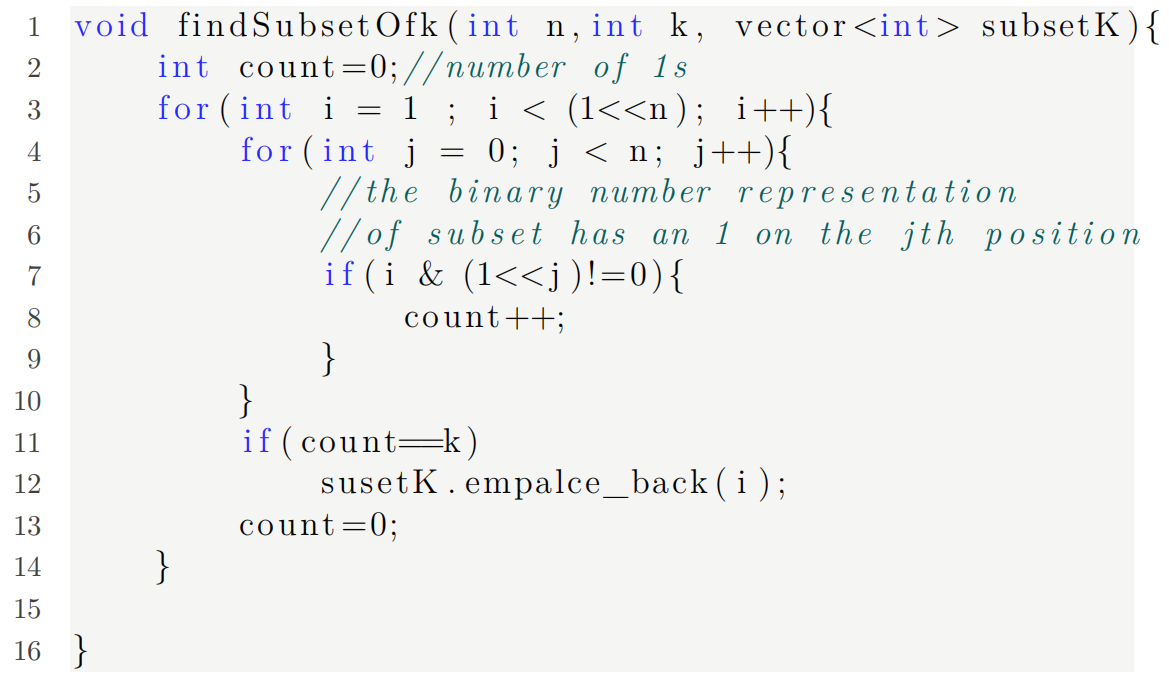
\includegraphics[width=11cm,height=6cm]{Figures/1.PNG}
\end{frame}

\begin{frame}{Basic Ideas}
    \begin{itemize}
        \item  However, we can easily find that the binary number representation of the subset whose number of elements is $k$ is no less than $2^k-1$. Therefore, we the code above, we can have an optimization on the $i$. The optimized code \textbf{findSubsetOfkOptim} is\\
        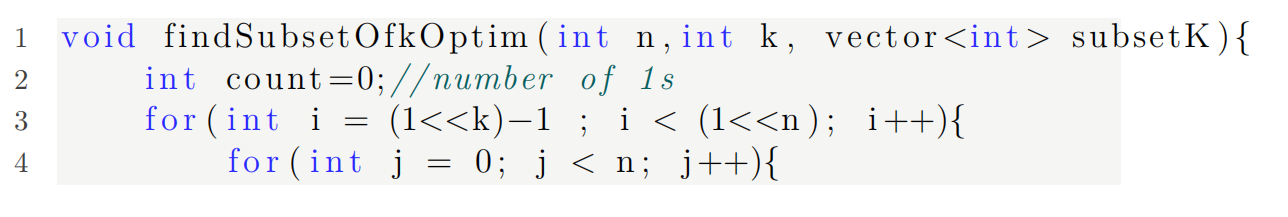
\includegraphics[width=11cm,height=2cm]{Figures/2.PNG}
    \end{itemize}
\end{frame}

\begin{frame}{Basic Ideas}
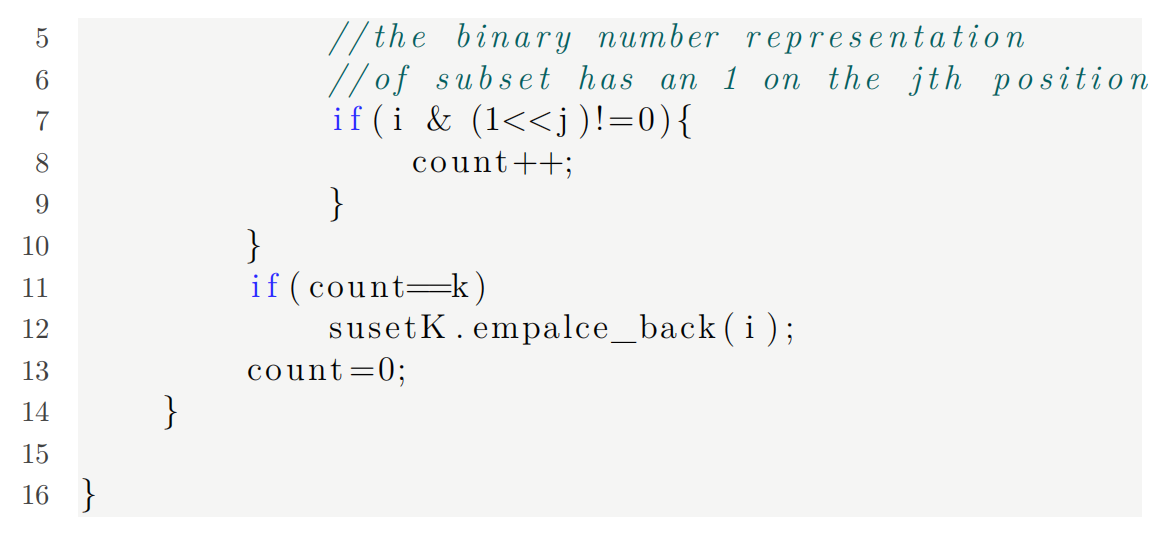
\includegraphics[width=10cm,height=4.5cm]{Figures/3.PNG}
    \begin{itemize}
        \item Currently, we can use the same way what we say above to find out the subset of the set whose number of element is $k$ and its number of elements is $s$.
    \end{itemize}
\end{frame}

\begin{frame}{Basic Ideas}
    \textbf{Calculate the Combination Number}\\
    If we calculate the combination number directly, it is likely to out of bounds of int. So we can use \textbf{combination formula}:
    \label{fol:C}$$C_n^m=C_{n-1}^{m-1}+C_{n-1}^m$$ 
    to calculate the combination number. And the specific implementation code can be seen in \textbf{calculateCombination}.\\
    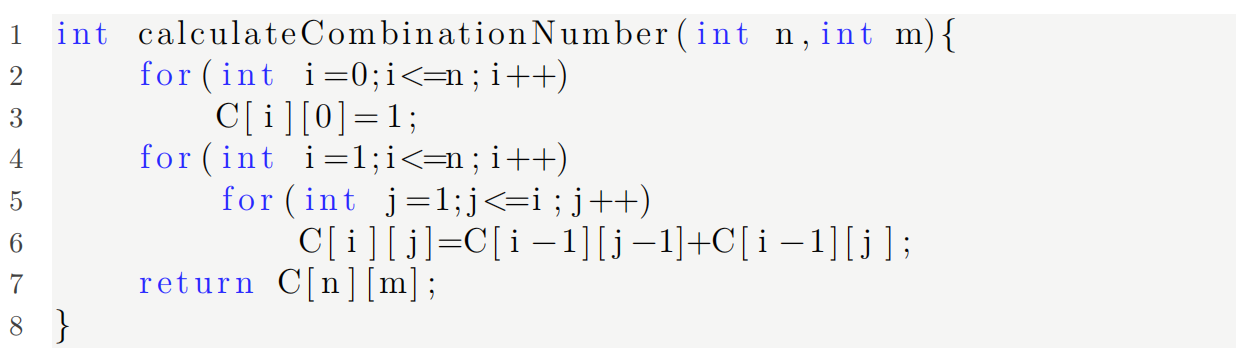
\includegraphics[width=10cm,height=3cm]{Figures/4.PNG}
\end{frame}

\begin{frame}{Basic Ideas}
    \textbf{Greedy Algorithm to Calculate the Set Coveraged}\\
    We denote that the input is a set $\mathcal{U}$ of n elements, and a collection $S=\{S_1, S_2, . . . , S_m\}$ of $m$ subsets of $\mathcal{U}$ such that $\cup_{i} S_i=\mathcal{U}$. Our goal is to take as few subsets as possible from $S$ such that their union covers $\mathcal{U}$. We can solve this problem easily by greedy algorithm. The algorithm is below in Table 3:
    \begin{center}
    \begin{table}[!hpbt]
        \begin{tabular}{|l|}
        \hline
        Greedy Cover($S$,$\mathcal{U}$)\\
        1. repeat\\
        2. pick the set that covers the maximum number of uncover element \\
        3.mark elements in the chosen set as covered\\
        4.remove the set from $S$ to the result set\\
        5. done\\ 
        \hline
        \end{tabular}
    \end{table}
    Table 3
    \end{center}
\end{frame}

\begin{frame}{Basic Ideas}
    Based on the three lemmas above, we can easily transform the problem to that the set $\mathcal{U}=\{1,2,\cdots, C^j_n\}$, which means that we map each different subset whose the number of the elements is j to a unique code from 1 to $ C^j_n$. Each subset of $S$, represents the each $k$ set's subsets whose number of elements is j. Ultimately, we can solve the problem easily.
\end{frame}

\begin{frame}{Basic Ideas}
    \textbf{When $j \neq s$:}\\
    The way to solve the problem is just like the way we mentioned above. However, after finishing finding the subset of the $k$ set whose element number is $s$, we should know how many sets whose the number of elements is $j$ include it. Therefore, we use \textbf{DFS(depth first search)} to find out them.\\
    Assuming that $n=5, s=3, j=4$, and the subset whose number of elements is equal to 3 is labeled as $01011_2$. Therefore, we can expand it as below in Table 4.
\end{frame}

\begin{frame}{Basic Ideas}
    \begin{center}
    \begin{table}[!hpbt]
        \centering
        \begin{tabular}{lllll}
        \hline
        \multicolumn{1}{|l|}{5} & \multicolumn{1}{l|}{4} & \multicolumn{1}{l|}{3} & \multicolumn{1}{l|}{2} & \multicolumn{1}{l|}{1}\\ \hline
        0& 1& 0& 1& 1\\
        0& 1& 1& 1& 1\\
        1& 1& 0& 1& 1                     
        \end{tabular}
    \end{table}
    Table 4
    \end{center}
    Then, we should mark the last two rows of the set above in the $\mathcal{U}$ as covered.
\end{frame}

\begin{frame}{Essential Codes and Functions Analysis}
    \textbf{Realization of Modifying DB files}\\
    As the request said, we need output the group of $k$ samples and corresponding result in DB files.\\
    First of all, we choose an OOP program language \textbf{C\#} which runs on\textbf{. Net framework} and\textbf{. Net core}(completely open source, cross platform) to help realize combine with modifying DB files.\\
    Depending on \textbf{C\#} powerful library and interface, we can apply our algorithm source code on GUI platform, and realizing the operation of creating new files(Code.1) as well as exporting result into corresponding files(Code.2).
\end{frame}

\begin{frame}{Essential Codes and Functions Analysis}
    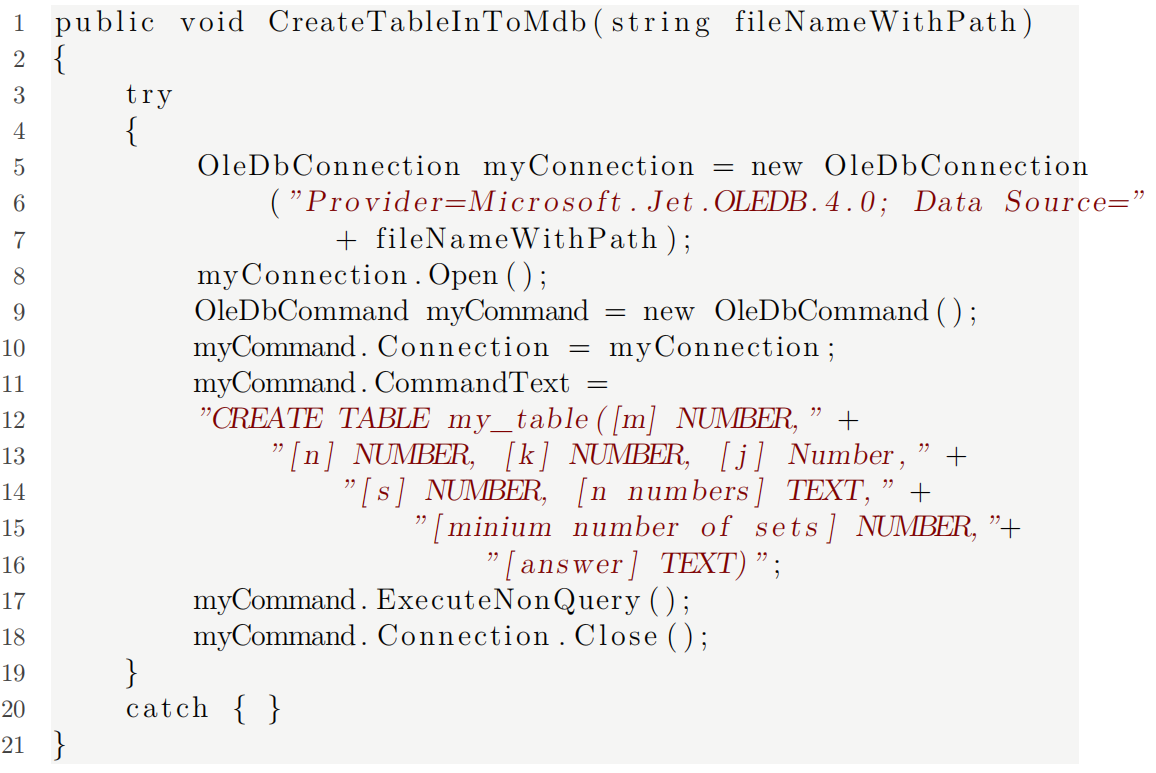
\includegraphics[width=11cm,height=7.5cm]{Figures/5.PNG}
\end{frame}

\begin{frame}{Essential Codes and Functions Analysis}
    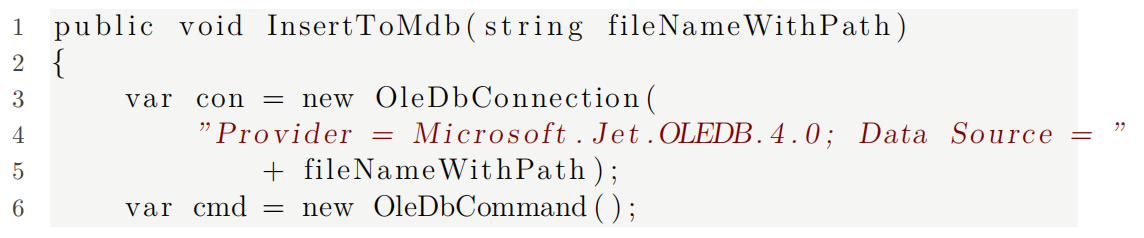
\includegraphics[width=11cm,height=2.5cm]{Figures/6.PNG}
\end{frame}

\begin{frame}{Essential Codes and Functions Analysis}
    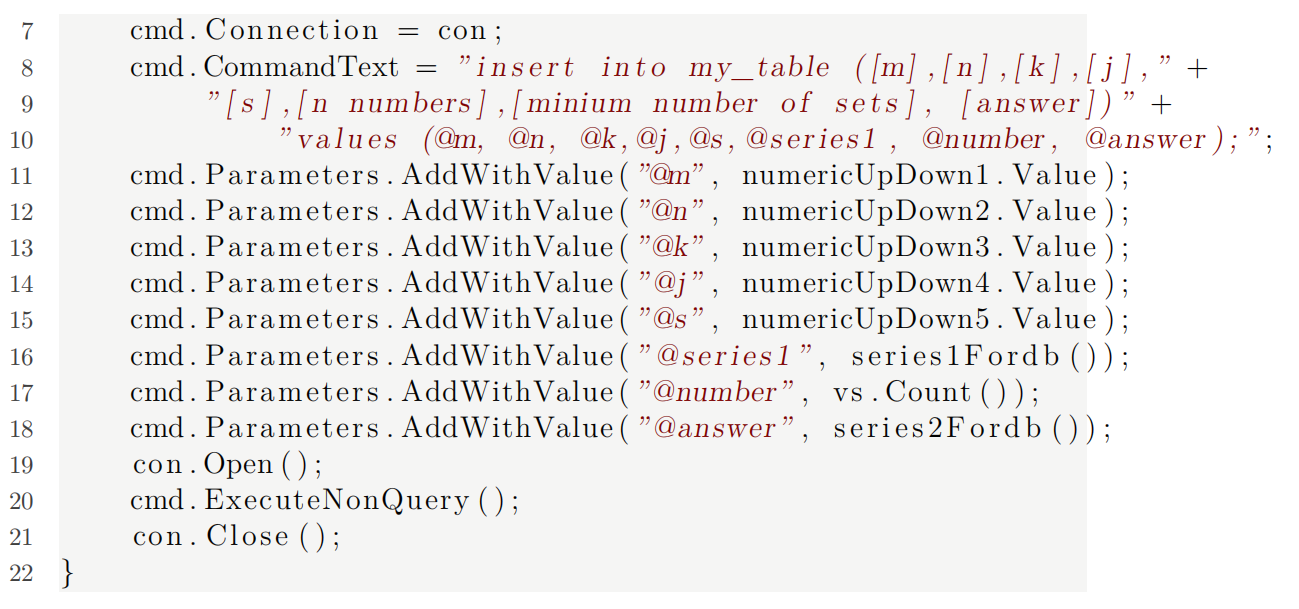
\includegraphics[width=11cm,height=6.5cm]{Figures/7.PNG}
\end{frame}

\begin{frame}{Essential Codes and Functions Analysis}
    \textbf{Multi-Threading}\\
    We adopt multi-threading programming way. We split the program into two parts, which are the GUI part and the calculation part. In this way, even if the program haven't figured out, the window of the program won't be stick. The specific implemented function is bound in \textbf{button2\_Click}.
\end{frame}

\begin{frame}{Essential Codes and Functions Analysis}
    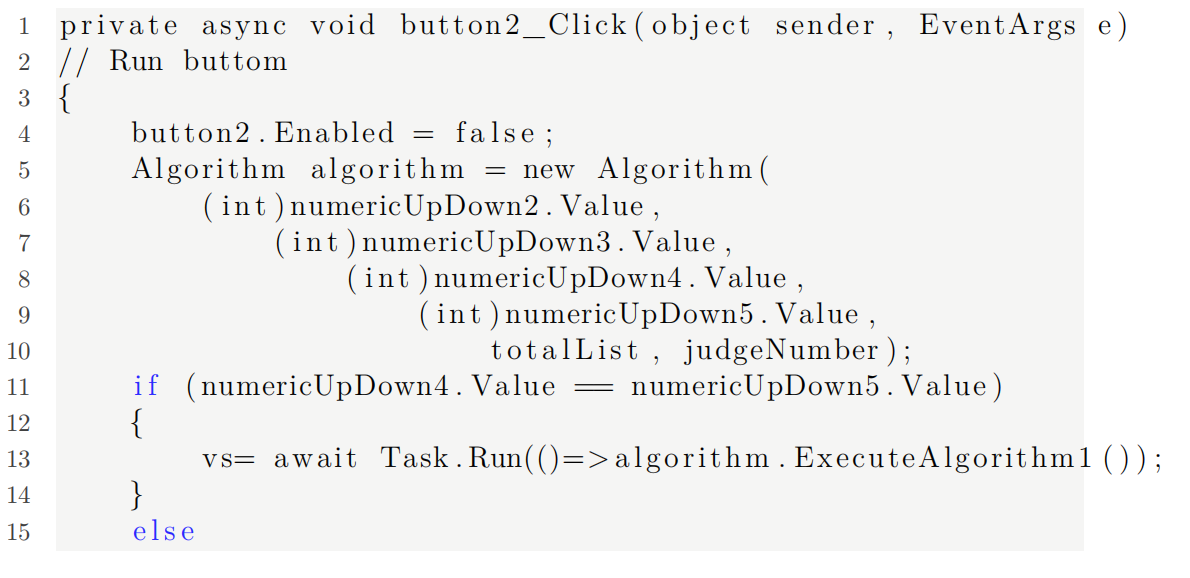
\includegraphics[width=11cm,height=6.5cm]{Figures/8.PNG}
\end{frame}

\begin{frame}{Essential Codes and Functions Analysis}
    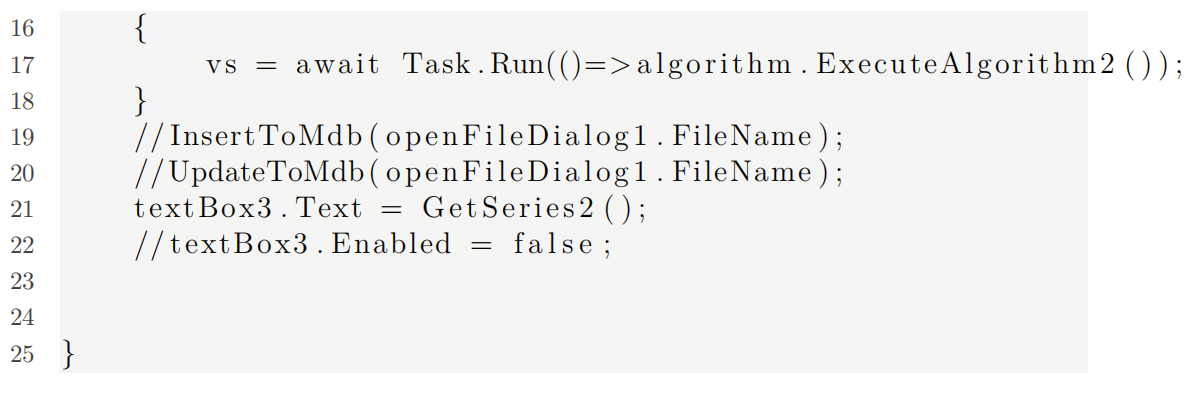
\includegraphics[width=11cm,height=4cm]{Figures/9.PNG}
\end{frame}

\begin{frame}{Program Test}
    The detailed steps that teach how to use program have been in the report. We just show the result in today's presentation.\\
    If the program window (Figure 1)can be displayed normally, you can enter the value for verification. The conditions of 1, 2, 3 and 4, 5 and 6, 7 in the project requirement file are similar, so we choose 1(Figure 2), 4(Figure 3), and 6(Figure 4) as the demo of our program.
\end{frame}

\begin{frame}{Program Test}
\begin{center}
    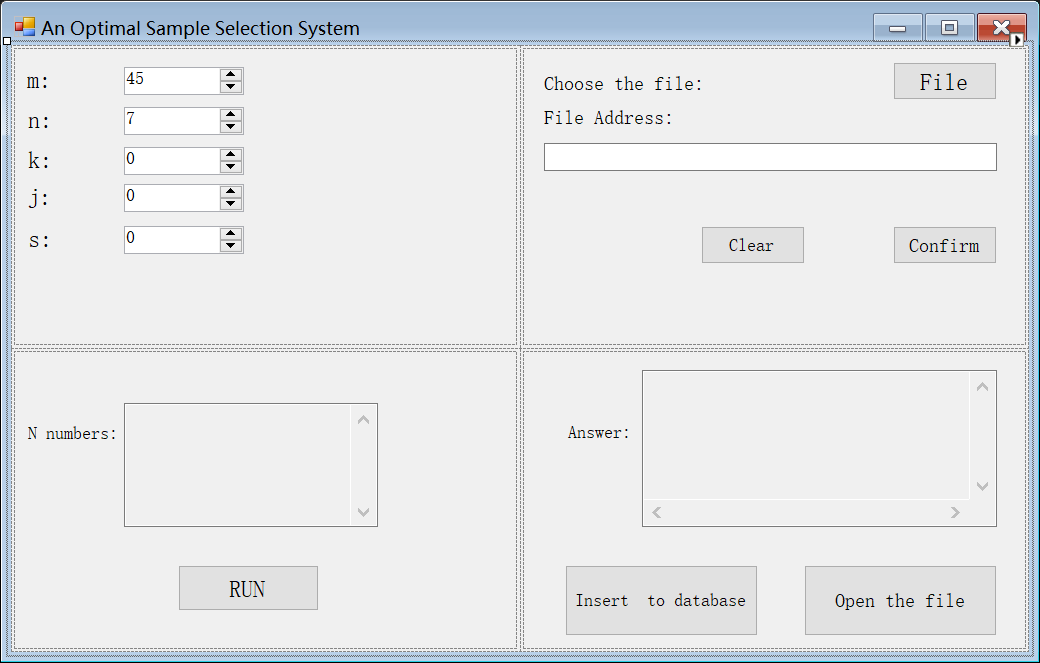
\includegraphics[width=8cm,height=6cm]{Figures/initial.png}\\
    Figure 1: initial program window
\end{center}
\end{frame}

\begin{frame}{Program Test}
\begin{center}
    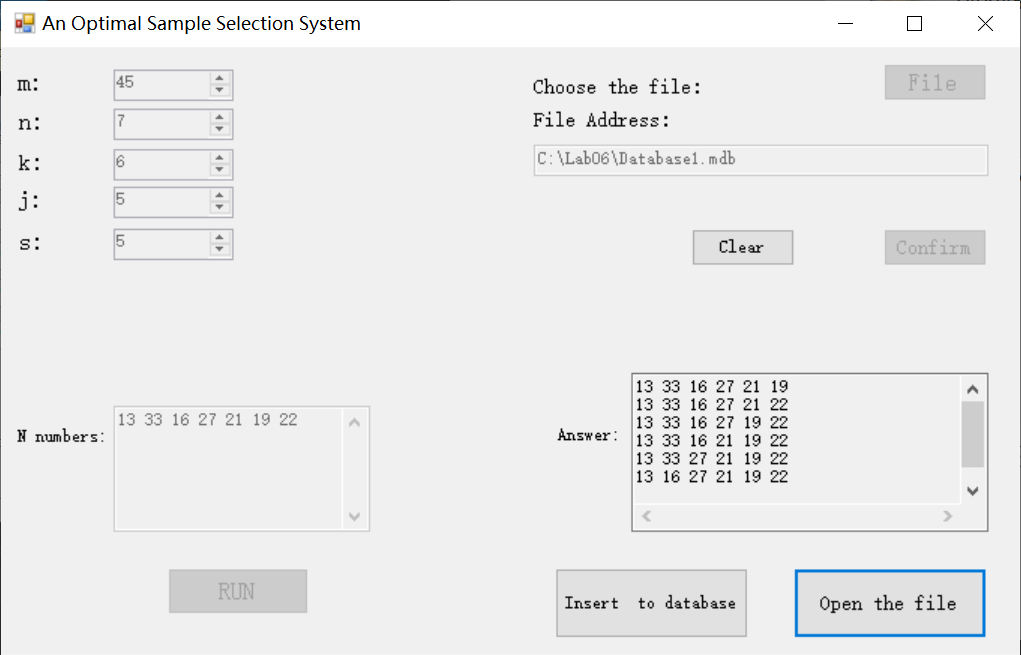
\includegraphics[width=8cm,height=6cm]{Figures/f1.png}\\
    Figure 2: E.g.$1$: Input the data: $m=45, n=7, k=6, j=5, s=5.$
\end{center}  
\end{frame}

\begin{frame}{Program Test}
\begin{center}
    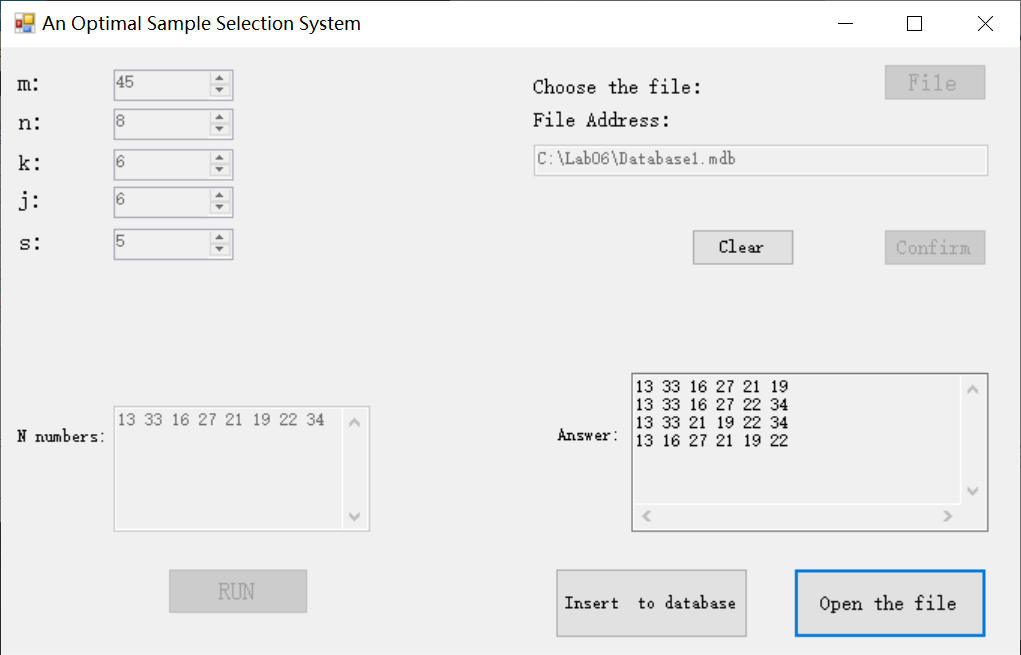
\includegraphics[width=8cm,height=6cm]{Figures/f4.png}\\
    Figure 3: E.g.$4$: Input the data: $m=45, n=8, k=6, j=6, s=5.$
\end{center}    
\end{frame}

\begin{frame}{Program Test}
\begin{center}
    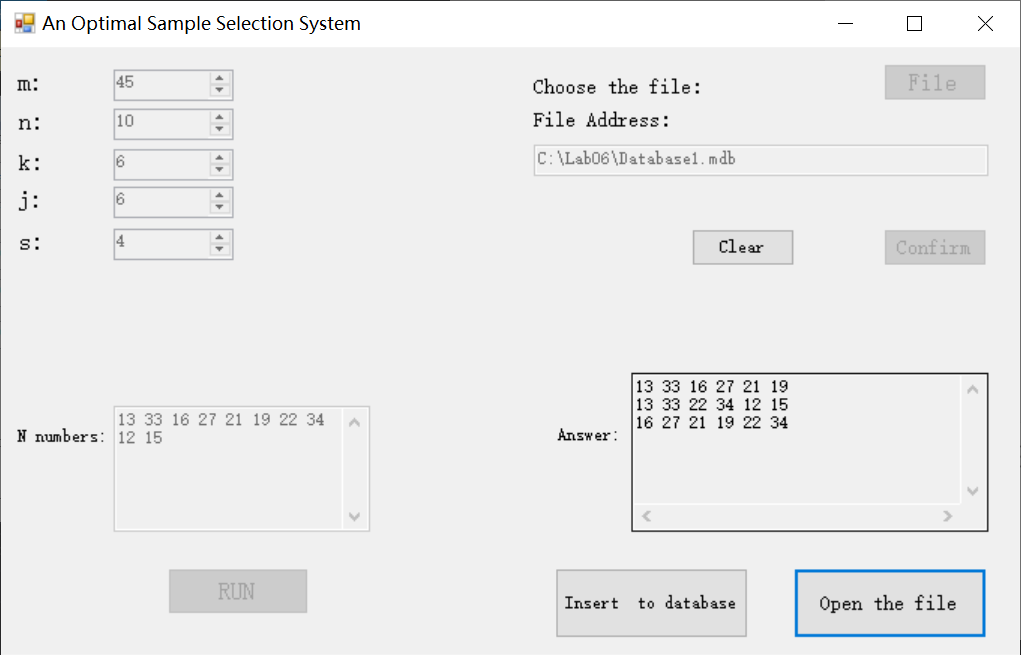
\includegraphics[width=8cm,height=6cm]{Figures/f6.png}\\
    Figure 4: E.g.$6$: Input the data: $m=45, n=10, k=6, j=6, s=4.$
\end{center}    
\end{frame}

\begin{frame}{Program Test}
    On-site test: The teacher can select values for random parameters, and we will test on site
\end{frame}

\begin{frame}{Summary}
    This project is based on the theoretical direction of \textbf{ME001} subject and combines some knowledge of data structure and mathematic, including optimal algorithms and combinatorics. But there are no correct understanding of some part of difficult and profound mathematic problems like fuzzy set. Authors point out about converse decimal digits to the binary make the big data abstraction in order to descend the time complexity. Besides, authors have already comprehend the core of program language \textbf{C\#} with utilizing \textbf{. Net Framework}. By using program, authors realize the process from theory to practice reflecting the theoretical view of unity of knowledge and practice. When writing large-scale projects, people often need cooperation and collaborative development, authors use \textbf{GitHub} for collaborative development and submit own patch code to collaborator's repository. In this article, we will utilize ideas to achieve team cooperation on \textbf{GitHub}.
\end{frame}

\begin{frame}{Summary}
    The last but not least, the goal of the future study and work is to work harder to learn this knowledge, in order to enrich, improve our level.
\end{frame}

\end{document}

